% (c) GreenSocs Ltd 2008
% author: Christian Schroeder <schroeder@eis.cs.tu-bs.de>

%%%%%%%%%%%%%%%
\section{Statistics Calculator}
\label{GAVStatisticsCalculator}

\ZwischenUberschrift{Concepts}
Most analysis tasks are performed by the {\em Statistics Calculator} (StatCalc) which is realized in the class \lstinline|StatCalc| in file \Datei{StatCalc.h}. The Statistics Calculator (class \lstinline|StatCalc|) manages the analysis of several 
input parameters that are calculated in a formula on several activation events. 
The tasks and the corresponding interfaces can be classified as follows:

\begin{enumerate}
  \item \textbf{Calculation Interface} (Calculator)\samepage
    \begin{itemize}
      \item Math operations
      \item Logical operations for boolean expressions usable as activation event
    \end{itemize}

  \item \textbf{Calculation Activation Events} (Trigger)
  \begin{itemize}
    \item Per default the result is updated (re-calculated) each time one of the {\em formula (input) parameter} changes.
    \item A boolean condition can guard the calculation. \newline 
    The calculation will only be performed if the given parameter is true. Note: A change of the condition parameter from false to true does not trigger re-calculation.
    \item A (complex) boolean expression can be created using another Statistics Calculator object giving its bool result parameter to \lstinline[language=TeX]|set_condition(gs_param<bool>&)|.
    \item An {\sffamily sc\_event} can be used to trigger the calculation. Each time the event is notified the calculation will be performed. (If there is a boolean condition activated this will be checked first.)
    \item A fixed interval, which triggers re-calculation each given time, can be specified.
    \item The calculation can also be manually performed by a simple function call.
  \end{itemize}

  \item \textbf{Statistics Abilities} (Calculator)
  \begin{itemize}
    \item {\em Sliding window}: The user can insert a sliding window between the calculation and the result. The sliding window puts out the average over the last $n$ values to the result parameter. \newline
    All activation mechanisms keep the same (parameter change callbacks, boolean conditions, {\sffamily sc\_event}, interval).
  \end{itemize}
\end{enumerate}

\begin{figure}[htbp]
	\centerline{
		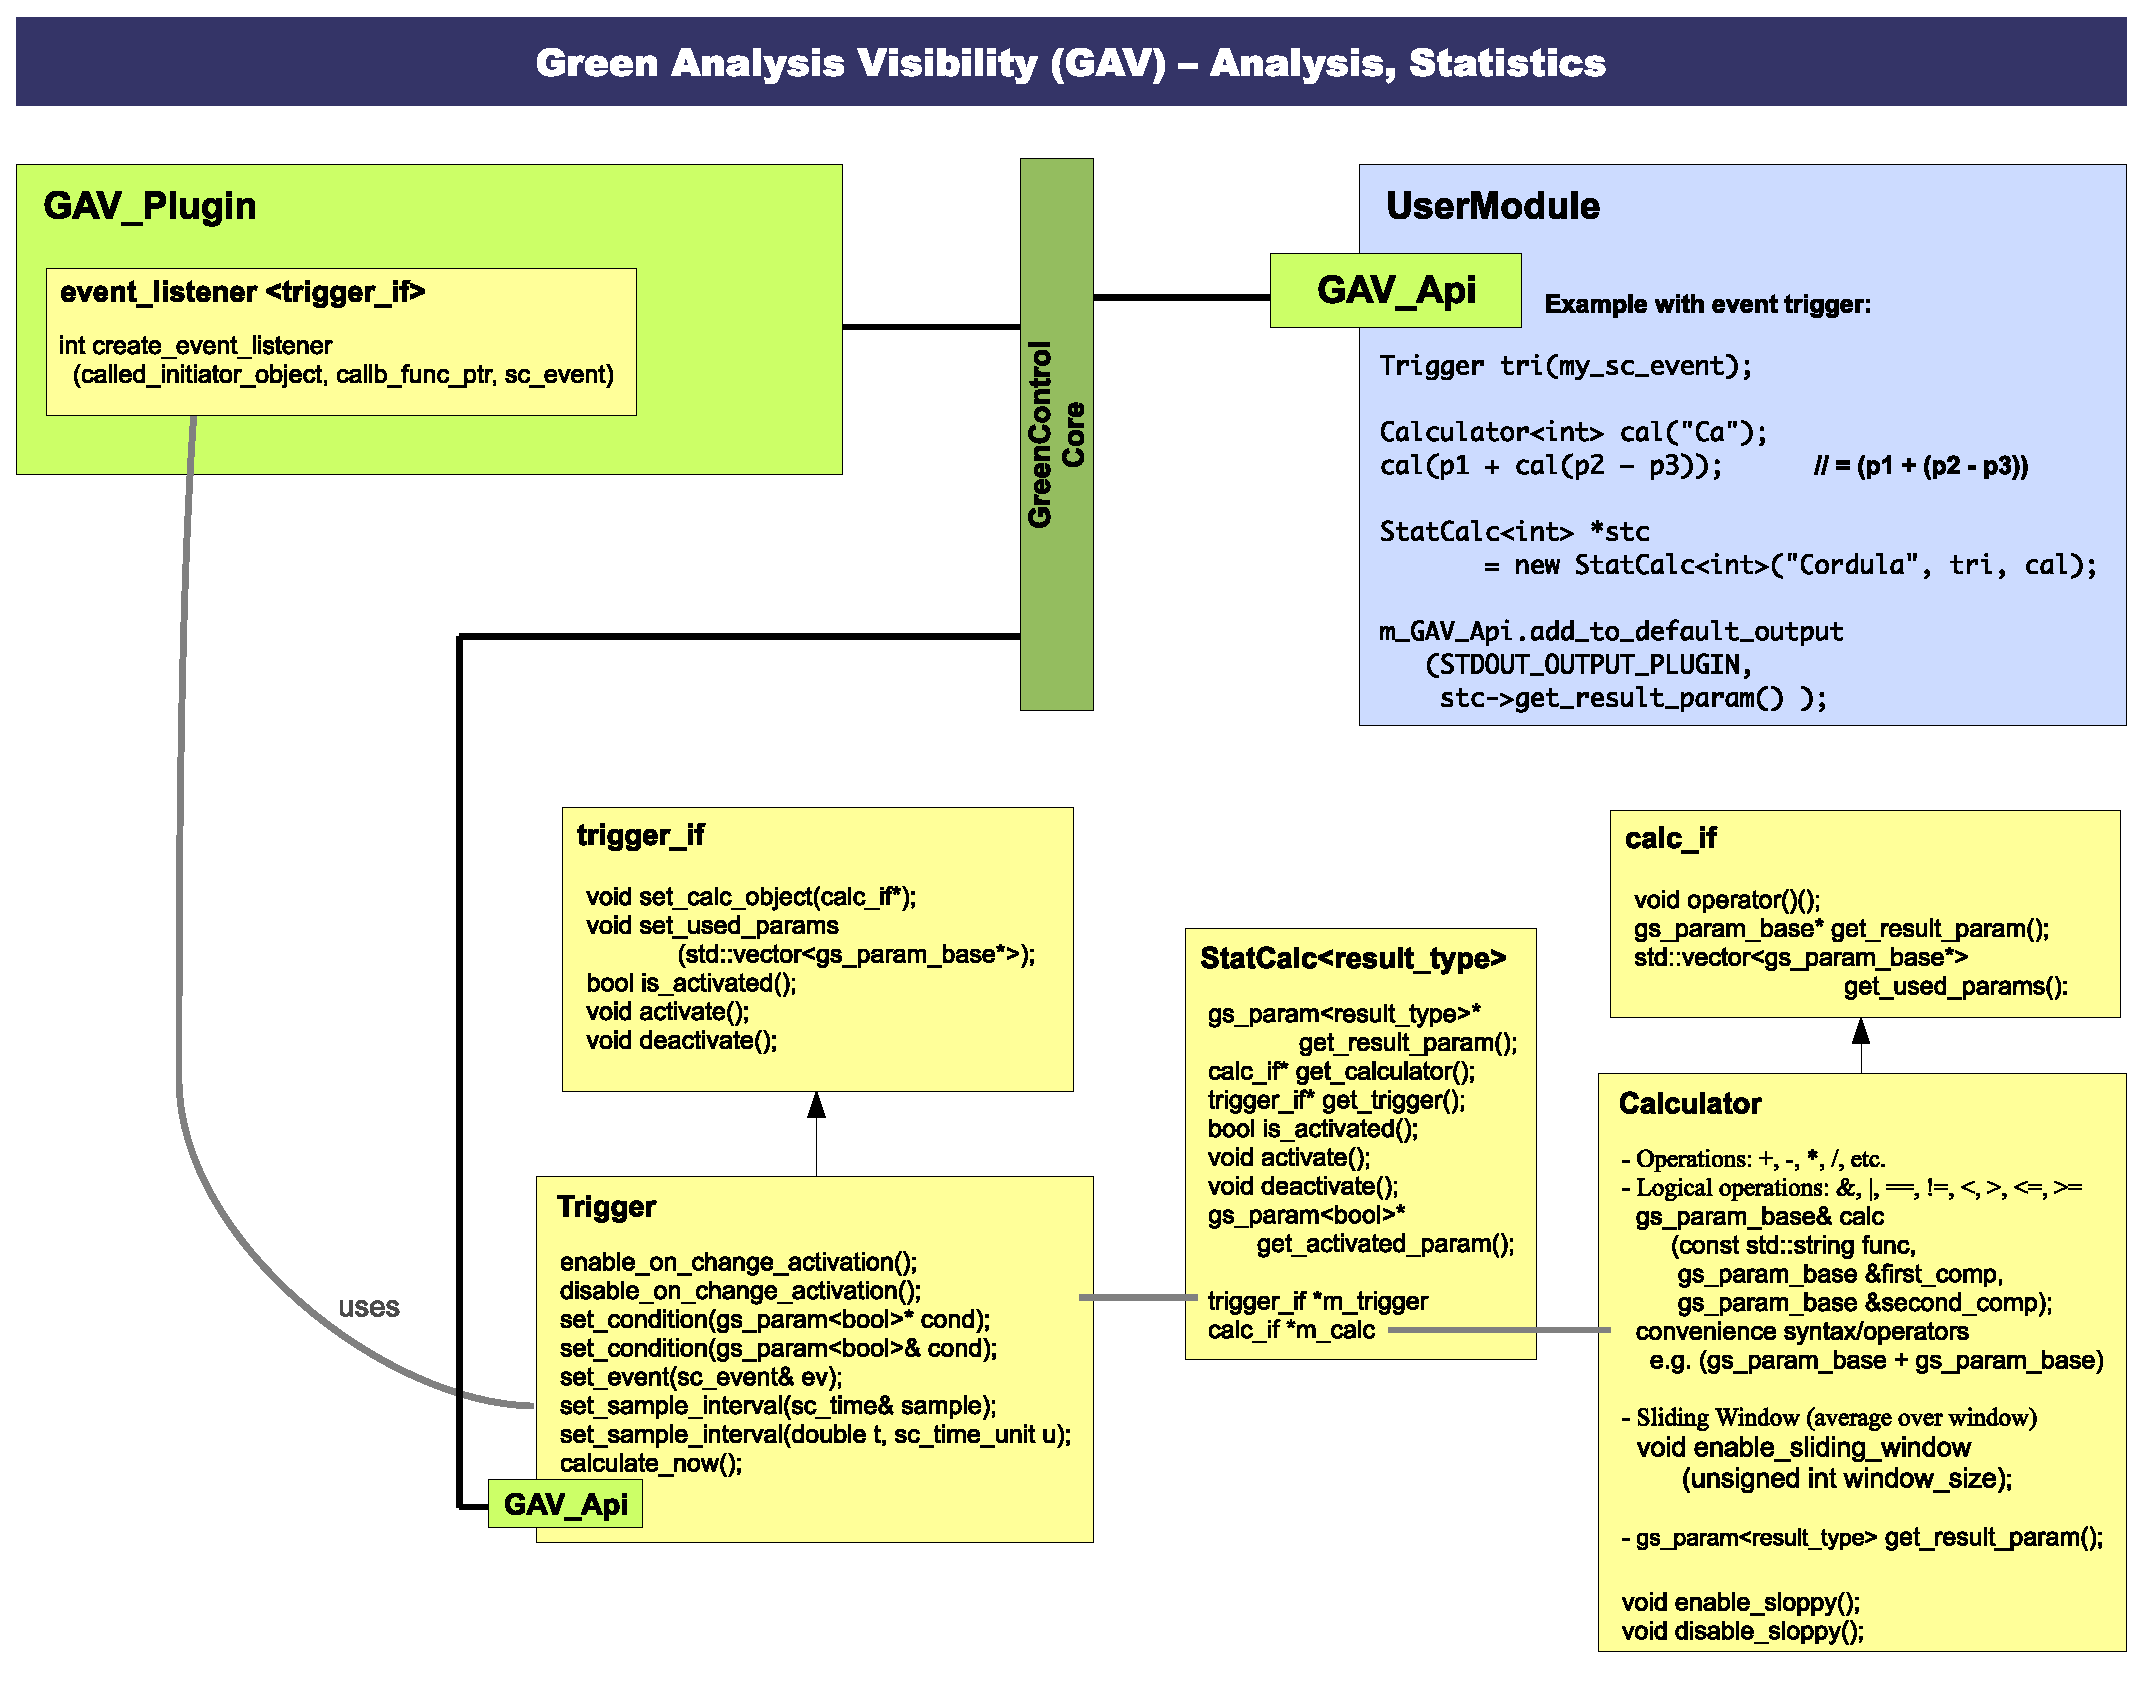
\includegraphics[width=\linewidth]{./images/GAVconcept(StatCalc)}}
	\caption{GreenAV Statistics Calculator Concept}
	\label{fig:GAVConceptStatCalc}
\end{figure}

Figure \ref{fig:GAVConceptStatCalc} shows the {\em Statistics Calculator concept}. The StatCalc consists mainly of a trigger object (see section \ref{GAVTrigger}) and a calculator object (see section \ref{GAVCalculator}). The calculator is responsible for managing the formula that should be calculated. The trigger manages the activation events of re-calculation and then calls the calculator to perform re-calculation.

The StatCalc object gets a trigger and a calculator object during construction and combines them. It gives the calculator functor object to the trigger object to enable the trigger to activate the recalculation. The StatCalc calls \lstinline|get_used_params()| on the calculator to give all input parameters to the trigger (using \lstinline|set_used_params()|.

\ZwischenUberschrift{Interface and how to use}
The \lstinline|StatCalc| object has to be instantiated {\em after} the trigger and calculator have been created and specified completely.

The {\em name} of the StatCalc has to be specified during construction and is made unique by the constructor using \lstinline|sc_gen_unique_name|.

The full constructors are:
\begin{lstlisting}
StatCalc(const char* stcalc_name, 
                        trigger_if* any_trigger, calc_if* any_calculator);
StatCalc(const char* stcalc_name, 
                        trigger_if& any_trigger, calc_if& any_calculator);
\end{lstlisting}

Alternative constructors do not need a trigger to be specified. In this case the default trigger object will we created by the StatCalc. The default trigger triggers on each input parameter change.
\begin{lstlisting}
StatCalc(const char* stcalc_name, calc_if* any_calculator);
StatCalc(const char* stcalc_name, calc_if& any_calculator);
\end{lstlisting}

The StatCalc object gives access to the trigger and calculator object pointers via the functions \lstinline|trigger_if* get_trigger()| and \lstinline|calc_if* get_calculator()| and provides some of the trigger and calculator interface functions whose calls will be redirected to the trigger object:
\begin{lstlisting}
gs_param<result_type>* get_result_param(); // redirected to calculator
calc_if* get_calculator(); // local
trigger_if* get_trigger(); // local
bool is_activated(); // redirected to trigger
void activate();     // redirected to trigger
void deactivate();   // redirected to trigger
\end{lstlisting}

The activation status of the trigger can also be accessed and manipulated with the parameter \mbox{\sffamily $<$statcalc\_name$>$.activated} which is returned by the function:
\begin{lstlisting}
gs_param<bool>* get_activated_param(); // local
\end{lstlisting}



%%%%%%%
\subsection{Trigger}
\label{GAVTrigger}

\ZwischenUberschrift{Concept}
The trigger is responsible for activation events. When one event occurs, the re-calculation of the calculator functor has to be called so the trigger object triggers the calculation. 

The trigger is an object that must inherit \lstinline|trigger_if| to allow it to be managed by the StatCalc object.

\ZwischenUberschrift{Interface}
All trigger classes have to implement the virtual interface \mbox{\lstinline|trigger_if|.} The following listing lists the functions to be implemented by a trigger class:

\noindent
\begin{minipage}{\textwidth}
\begin{lstlisting}[caption={Trigger interface trigger\_if}]
class trigger_if {
  virtual ~trigger_if() { }
  // Initialization functions
  virtual void set_activated_param(gs::gs_param<bool> &activated) = 0;
  virtual void set_calc_object(calc_if*) = 0;
  virtual void set_used_params(std::vector<gs_param_base*>) = 0;
  // User functions
  virtual bool is_activated() = 0;
  virtual void activate() = 0;
  virtual void deactivate() = 0;
  // Callback functions
  virtual void event_callback() = 0;
  virtual void interval_callback() = 0;
};
\end{lstlisting}
\end{minipage}

For a detailed description see the \hyperlink{GAVDoxygenRef08target}{API reference}.

The initialization functions are called by the StatCalc during its construction.

The function \lstinline|set_activated_param| gets a reference to the parameter that has been created by the StatCalc and which represents and modifies the activation status. The trigger has to register a callback for this parameter to react on changes. This function is called before the other initialization functions to ensure that the parameter is available.

The function \lstinline|set_used_params| gets the formula parameters of the calculator. These parameters have to be observed by the trigger for destruction. After one of these parameters has been destructed the trigger must never again call the re-calculation of the calculator!

The function \lstinline|deactivate| should deactivate the trigger until the function \lstinline|activate| is called. A deactivated trigger should unregister all input parameter callbacks (for changes and destruction checks) due to performance reasons: A deactivated trigger should produce no overhead! This allows creation of (deactivated) Statistics Calculators without runtime overhead. Get if the trigger is activated by calling \lstinline|is_activated|.

The functions \lstinline|event_callback| and \lstinline|interval_callback| are both functions that can be registered by the trigger to the event listener of the GAV plugin (which may be accessed via the \lstinline|GAV_Api|) which is templated to \lstinline|trigger_if|.

\Note{Advanced Note}{Re-implement a trigger}{
  As an extension to the \GreenAV framework new triggers can be implemented. They just have to implement the \lstinline|trigger_if| interface.
  
  This may be needed if further activation events are needed that are not met by the default \GreenAV trigger.
  
  When re-implementing a trigger be careful never calling the re-calculation if one of the formula parameters has been destroyed. Also take care to deactivate the trigger completely when the deactivation function is being called. On activation you have to check whether all formula parameters are still existing.
}

\ZwischenUberschrift{GreenAV default Trigger and calculation activation events}

The default {\em GreenAV trigger} object class is \lstinline|Trigger|.

The trigger automatically registers for callbacks of all formula (input) parameters which are given to the trigger via the \lstinline|set_used_params| call. The trigger handles destructed input parameters by deactivating the trigger forever and never again calling the calculator functor object. Even if parameter changes are not a calculation activating event, the trigger registers for callbacks just to check if the changed parameter is being destructed.

\textbf{Calculation activation event kinds} this Trigger supports are:
\begin{itemize}
  \item sc\_event for {\em SystemC events}: \vspace{.5em} \newline 
  The sc\_event calculation activation event uses the trigger event listener of the GAV plugin to wait for the user-given event. When the event is notified the trigger will be called back (function \lstinline|event_callback|) by the event trigger.

  \item sc\_time for {\em periodical sample intervals} (periodically repeated events)  \vspace{.5em} \newline 
  The sc\_time calculation activation event notifies the trigger itself periodically after the specified time intervals. This trigger also uses the API's event listener. This may be used e.g. for sliding windows that record on fixed time intervals.
  
  \item {\em value changes} on input parameters (uses parameter callbacks)  \vspace{.5em} \newline 
  This is the {\em default} trigger mechanism. The trigger registers callbacks for all formula input parameters and triggers re-calculation an each callback.
  
  \item {\em manually chosen parameter changes}
   The user may give any gs\_params to the trigger whose value changes will result in a re-calculation. These parameters need not (but may) be formula parameters.
  
  \item {\em manually}  \vspace{.5em} \newline
  The user may manually trigger the re-calculation with a simple function call.
\end{itemize}

\textbf{Additionally} the Trigger supports a
\begin{itemize}
  \item {\em Guard} ({\em no} activation event): \lstinline[language=TeX]|gs_param<bool>| for a condition to be checked before calculation.  \vspace{.5em} \newline 
  This guard parameter is checked each time the trigger got one of the activation events. If the guard's value is {\sffamily true} the re-calculation is performed, otherwise re-calculation is suppressed.
\end{itemize}

The trigger is able to handle several activation events concurrently. The user may enable value change activation and e.g. set one (or more) sc\_event(s) on whose notification triggering will also be performed. Manually triggering is always possible (taking account of the guard as well).

\Note{Implementation Note}{Event listener}{
  The trigger needs the API's event listener templated to \lstinline|trigger_if|. During construction the trigger gets a \lstinline|GAV_Api| instance and calls \lstinline|get_event_listener| and stores the pointer. 
  \vspace{.5em}

  Afterwards the trigger calls \lstinline|m_event_listener->create_event_listener(this, &trigger_if::event_callback, ev);| where it is needed to create a dynamically spawned process that waits for the event \lstinline|ev|.
}

\ZwischenUberschrift{How to use}
This section is about how to prepare the trigger in the user's code before giving it to the \lstinline|StatCalc| object.

The specific constructors specify the way the trigger waits for calculation activation events. The vector parameter takes manually chosen parameters. There are constructors for many combinations of activation events:
\begin{lstlisting}[caption={Trigger constructors with several calculation activation events and guard}]
explicit Trigger();
explicit Trigger(sc_event& event);
explicit Trigger(sc_event* event);
explicit Trigger(sc_time ti);
explicit Trigger(double t, sc_time_unit u);
explicit Trigger(bool on_changes);
explicit Trigger(sc_event& event, gs_param<bool> &cond);
explicit Trigger(sc_time &ti, gs_param<bool> &cond);
explicit Trigger(double t, sc_time_unit u, gs_param<bool> &cond);
explicit Trigger(bool on_changes, gs_param<bool> &cond);
explicit Trigger(gs_param<bool> &cond);
explicit Trigger(gs_param<bool> *cond);
explicit Trigger(sc_event &ev, sc_time &ti, bool on_changes, 
                 gs_param<bool> cond);
explicit Trigger(sc_event &ev, sc_time &ti, gs_param<bool> &cond);
explicit Trigger(sc_event &ev, sc_time &ti);
explicit Trigger(sc_event &ev, bool on_changes);
explicit Trigger(sc_time &ti, bool on_changes, gs_param<bool> &cond);
explicit Trigger(sc_time &ti, bool on_changes);
explicit Trigger(std::vector<gs_param_base*>);
\end{lstlisting}

The constructor activation event and guard order is: 
{\sffamily sc\_event}, {\sffamily sc\_time}, {\sffamily bool\_on\_changes}, {\sffamily guard}.

There may be activation event combinations which are not available, e.g. when combining manually chosen parameters with other event.Then the user may use one constructor and one of the following functions after construction: 
\begin{itemize}
  \item \lstinline|set_event(sc_event& ev)| enables trigger for SystemC events.  \vspace{.5em} \newline
    When called repeatedly all events are valid. Removing events is not possible.
  \item \lstinline|set_sample_interval(sc_time& sample)| enables periodical sample interval trigger.  \vspace{.5em} \newline
    When called repeatedly the last interval is the valid one.
  \item \lstinline|enable_on_change_activation()| enables trigger for value changes,  \vspace{.5em} \newline
    \lstinline|disable_on_change_activation()| may be used to disable the value change trigger while the trigger 'runs'.
  \item \lstinline[language=TeX]|set_condition(gs_param<bool>* cond)| or \lstinline[language=TeX]|set_condition(gs_param<bool>& cond)| sets the guard parameter.   \vspace{.5em} \newline
    \lstinline|cond = NULL| removes the guard. \newline
    When being called repeatedly the old guard will be overwritten.
\end{itemize}
All these functions may be called anytime (even if trigger already 'runs').
 
Further available functions are:
\begin{itemize}   
  \item \lstinline|calculate_now()| triggers the re-calculation manually. This call takes account of the activation and the guard just like all activation events do. 
  \item \lstinline[language=TeX]|bool is_activated()| returns if the trigger / StatCalc is activated, see interface description above.
  \item \lstinline[language=TeX]|void activate()| activates the trigger / StatCalc, see interface description above.
  \item \lstinline[language=TeX]|void deactivate()| deactivates the trigger / StatCalc, see interface description above.
  \item \lstinline[language=TeX]|void set_activation_status(bool _activate)| calls \lstinline|activate| or \lstinline|deactivate|.
\end{itemize}

The following listings are some usage examples:

For the example this predefinitions are needed:
\begin{lstlisting}
#include "greencontrol/analysis.h"
\end{lstlisting}

\vspace{.5cm}

\begin{lstlisting}[caption={Example: standard value change trigger.}]
gs::av::Trigger *stc_tom_t = new Trigger(true);
  // is the same as 
gs::av::Trigger *stc_tom_t = new Trigger();
\end{lstlisting}

\begin{lstlisting}[caption={Example: standard value change trigger with condition guard.}]
gs::gs_param<bool> condition("condition");
gs::av::Trigger stc_regina_t(condition); // uses param changes and a guard
'... create calculator, StatCalc ...'
'... do something ...'
// disable standard value change trigger
stc_regina_t.disable_on_change_activation();
'...'
stc_regina_t.calculate_now(); // calculate manually
'...'
stc_regina.deactivate(); // deactivates the trigger
'...'
stc_regina.activate(); // re-activates the trigger
\end{lstlisting}

\begin{lstlisting}[caption={Example: SystemC event trigger.}]
sc_event event0;
gs::av::Trigger stc_cordula_t(event0);
'...'
event0.notify(); // will trigger
\end{lstlisting}

\begin{lstlisting}[caption={Example: periodical sample interval trigger.}]
gs::av::Trigger stc_bob_t(10, SC_NS);
'...'
stc_bob_t.set_sample_interval(0, SC_NS); // removes trigger
\end{lstlisting}

See files \Datei{AVnewStCalc.*} in the example \Verzeichnis{greencontrol/examples/gav\_StatCalc/} for regression tests on the trigger.




%%%%%%%
\subsection{Calculator}
\label{GAVCalculator}


%%%
\ZwischenUberschrift{Concept}
The calculator functor object is responsible for performing the calculation defined by the user.
The calculator is an object that inherits \lstinline|calc_if| to allow to be managed by the StatCalc object. It performs the calculation when the \lstinline[language=TeX]|operator()| is called by the trigger.

The default {\em GreenAV calculator} object class is \lstinline|Calculator|. 


%%%
\ZwischenUberschrift{Interface}
As an extension to the \GreenAV framework new calculators can be implemented which just have to implement the virtual interface \lstinline|calc_if|:
 
\noindent
\begin{minipage}{\textwidth}
\begin{lstlisting}[caption={Calculator interface calc\_if}]
class calc_if {
  virtual ~calc_if() { }
  void operator()() = 0;
  gs_param_base* get_result_param() = 0;
  std::vector<gs_param_base*> get_used_params() = 0;
};
\end{lstlisting}
\end{minipage}

For a detailed description see the \hyperlink{GAVDoxygenRef08target}{API reference}.

The function \lstinline|operator()| enables the calculator object to be a functor. This function performs the calculation regardless of the formula input parameter status. The trigger has to make sure not to call the function if the calculation will fail (e.g. because of destructed formula parameters).

The function \lstinline|get_result_param| returns a pointer to the result parameter. The result parameter is created and owned by the calculator. This function should not be called before the formula was specified.

The function \lstinline|get_used_params| is called by the StatCalc during construction and returns all formula input parameters to be given to the trigger. These parameters are needed by the trigger for checking the destruction callbacks and -- if activated -- for the parameter change callbacks.

\Note{Advanced Note}{Re-implement a calculator} {
  As an extension to the \GreenAV framework new calculators can be implemented. They just have to implement the \lstinline|calc_if| interface.
  
  This may be needed if other calculations shall be available, e.g. calculate within a script language instead using SystemC~/~C++. If only further functions consuming two parameters are needed, user defined functions can be added to the default \GreenAV calculator, see below.
}


%%%
\ZwischenUberschrift{GreenAV default Calculator}
The default {\em GreenAV calculator} object class is \lstinline|Calculator| (and \lstinline|Calculator_bit|).

\textbf{Features} of the Calculator:
\begin{itemize}
  \item Variable data type of the Calculator's result and intermediate results:  \vspace{.5em} \newline
  	The template parameter of the Calculator class specifies the type of all operations, intermediate 
	results and the result parameter. All formula parameters will be casted to this type for each operation.
  \item Formulas with various, nested operations can be built with formula input parameters \newline
	(of type \lstinline|gs_param<T>|):
	\begin{itemize}
	  \item Math operations 
		\colorbox{hellgrau}{$+$}, \colorbox{hellgrau}{$-$}, \colorbox{hellgrau}{$/$}, \colorbox{hellgrau}{$*$},
	  \item Logical operations
	  	\colorbox{hellgrau}{$==$}, \colorbox{hellgrau}{$!=$}, \colorbox{hellgrau}{$>=$}, 
		\colorbox{hellgrau}{$<=$}, \colorbox{hellgrau}{$<$}, \colorbox{hellgrau}{$>$},
	  \item Bitwise operations 
	  	\colorbox{hellgrau}{$\&$}, \colorbox{hellgrau}{$|$} 
		(in the derived class \lstinline|Calculator_bit|), \vspace{.5em} \newline
	           \WarningSymbol{} Some data types are not allowed to have bitwise operations, accordingly 
	           they are not included in the \lstinline|Calculator| class. If these operations should be used, 
	           use the class \lstinline|Calculator_bit| instead!
	\end{itemize}
  \item Calc-syntax (\lstinline|calc(string, gs_param<T>, gs_param<T>)|) for flexible and powerful 
  	formula creation: \vspace{.5em} \newline
	This is the main part of the calculator: the mechanism to specify formulas. Use the string 
	to specify the operation, the input parameters may be results of another calc-call. 
	Calls to \lstinline|calc| can be nested.
  \item Convenient operators \colorbox{hellgrau}{$+$}, \colorbox{hellgrau}{$-$}, 
  	\colorbox{hellgrau}{$/$}, \colorbox{hellgrau}{$*$} 
	(less flexible and powerful but better human-readable) for parameter bases: \vspace{.5em} \newline
	The convenient operators may be used to replace the calc-syntax for the math operations. 
  \item User defined functions for calc-syntax: \vspace{.5em} \newline
  	It is simple to add user defined functions including their operation strings to a Calculator of 
	specified type. This may be done e.g. in the {\sffamily sc\_main}. A function added to 
    \lstinline|Calculator<type>| is also available in \lstinline|Calculator_bit<type>|.
  \item Constants in formula:  \vspace{.5em} \newline
  	Using the calc-syntax hard-coded constants may be used instead of parameters.
  \item Statistics: sliding window: \vspace{.5em} \newline
  	The sliding window can be activated after the formula has been specified completely. The sliding window gets a window size ($n$). The function will add the results of the last $n$ calculations and divide this by the window size $n$.
  \item Switch to allow {\em sloppy calculations}:  \vspace{.5em} \newline
  	A special feature of the \GreenAV Calculator is the ''sloppy'' functionality.
	The user may enable sloppy behavior to pretend runtime errors, e.g. when dividing by zero. Each 
	operation may define a default return value if sloppy is enabled. E.g. if sloppy is enabled the division
	(\colorbox{hellgrau}{$/$}) operation returns $0$ if divided by zero.
\end{itemize}

The Calculator's formula parameters are {\em limited} to these POD and SystemC {\em data types}: \newline
   \lstinline[language=TeX]|int|,
   \lstinline[language=TeX]|unsigned int|,
   \lstinline[language=TeX]|bool|,
   \lstinline[language=TeX]|double|,
   \lstinline[language=TeX]|float|,
   \lstinline[language=TeX]|unsigned long long|,
   \lstinline[language=TeX]|unsigned char|,
   \lstinline|sc_int_base|,
   \lstinline|sc_int|,
   \lstinline|sc_uint_base|,
   \lstinline|sc_uint|,
   \lstinline|sc_signed|,
   \lstinline|sc_bigint|,
   \lstinline|sc_unsigned|,
   \lstinline|sc_biguint|.  \newline
The data types are identified by the parameter call \lstinline|getType| which returns the type as an enum {\sffamily gs::cnf::Param\_type}, see file \Datei{gcnf\_datatypes.h}.

If parameters of type \lstinline|sc_time| should be used as input parameters, a Calculator of type \lstinline[language=TeX]|double| should be used.

The Calculator does {\em no} initial calculation when being created! This assures that only when the specified activation events occur the calculation will be performed.

%%%
\ZwischenUberschrift{How to use}
The steps before adding a calculator to the StatCalc's constructors are:
\begin{enumerate}
  \item Create a \lstinline|Calculator| (or \lstinline|Calculator_bit|) object giving a name to the constructor.
  \item Specify the formula which this calculator should use. Use the calc-syntax or the convenient operators.
  \item Optional: get the result parameter. This may also be called on the StatCalc object after having created it.
\end{enumerate}

%%
\paragraph{Calc-syntax}
The {\em calc-syntax} is the designated way of setting up a complex formula of several formula input parameters. A \lstinline|calc|-call gets as function call parameters a string specifying the operation and two input parameters of type \lstinline|gs_param<T>| or \lstinline|gs_param_base|. Nested calls of \lstinline|calc| function calls may be used because the \lstinline|calc| function returns an intermediate result parameter. 

The listings \ref{lst:GAVCalcEx1} and \ref{lst:GAVCalcEx2} show examples how to specify a calculation formula using the calc-syntax.

\noindent
\begin{minipage}{\textwidth}
\begin{lstlisting}[caption={
	Simple example using the calc-syntax: \newline 
	Calculator type: {\sffamily unsigned long long}, formula: $(scint + scbuint)$.
	}, label=lst:GAVCalcEx1]
gs::gs_param<sc_int<10> > scint("scint", 10); 
gs::gs_param<sc_biguint<70> >scbuint("scbuint", 10);

gs::av::Calculator<unsigned long long> c("my_calc");
c.calc("+", scint, scbuint);
\end{lstlisting}
\end{minipage}

\noindent
\begin{minipage}{\textwidth}
\begin{lstlisting}[caption={
	Example using the calc-syntax: \newline 
	Calculator type: {\sffamily double}, formula: $(((int\_p - int\_p2) / int\_p2) + (dbl\_p * uint\_p))$.
	}, label=lst:GAVCalcEx2]
gs::gs_param<double> dbl_p("dbl_p"); gs::gs_param<int> int_p("int_p"); 
gs::gs_param<int> int_p2("int_p2");
gs::gs_param<unsigned int> uint_p("uint_p");

gs::av::Calculator<double> c1("my_calculator");
c1.calc("+", c1.calc("/", c1.calc("-", int_p, int_p2), 
                          int_p2), 
             c1.calc("*", dbl_p, uint_p));
\end{lstlisting}
\end{minipage}

%\begin{center}
%\setlength{\fboxrule}{.5pt}
%\setlength{\fboxsep}{1em}
%\fbox{
%\begin{minipage}{15cm}
\paragraph{Convenient operators}
%\begin{itemize}
  %\item 
  Alternative to the calc function you may use more {\em convenient operators}: \newline
  For the operations \colorbox{hellgrau}{$+$}, \colorbox{hellgrau}{$-$}, \colorbox{hellgrau}{$/$}, \colorbox{hellgrau}{$*$} there are operators for the \lstinline|gs_param_base| class. See listing \ref{lst:GAVConvOpEx} for an example, listing \ref{lst:GAVMixedOpEx} shows how to mix convenient operators with calc-syntax. \newline
  You may use \lstinline|c( c(i1 + i2)  +  c(i2 * i2)| where i1 and i2 have to be \lstinline|gs_param_base|s!
    \begin{list}{\WarningSymbol{Warning:}} {\setlength{\leftmargin}{2.3cm}  \setlength{\labelwidth}{3cm}  }
      \item Be careful to surround each operation with a calculator call: \newline
               \lstinline[language=TeX]|my_calculator(<param_base> <operator> <param_base>)|!
      \item Only parameter bases (\lstinline|gs_param_base|) may be used, \newline 
               no \lstinline|gs_param<T>|!
    \end{list}
  %\item 
%\end{itemize}
%\end{minipage}
%}
%\end{center}

\noindent
\begin{minipage}{\textwidth}
\begin{lstlisting}[caption={
	Example using convenient operators: \newline 
	Calculator type: {\sffamily int}, formula: $(b1 - (b1+b2)) + ((b1*b2) / b2)$.
	}, label=lst:GAVConvOpEx]
gs::gs_param_base &b1 = int_p; // int_p gs_param<int>, see example above
gs::gs_param_base &b2 = int_p2; // int_p2 gs_param<int>, see example above
gs::gs_param_base &bu3 = uint_p; // uint_p gs_param<uint>, see expl. above

gs::av::Calculator<int> cc("my_convCalc");
cc(cc(b1 - cc(b1 + b2)) + cc(cc(b1 * b2) / b2));
\end{lstlisting}
\end{minipage}

\noindent
\begin{minipage}{\textwidth}
\begin{lstlisting}[caption={
	Example mixing calc-syntax and convenient operators: \newline 
	Calculator type: {\sffamily int}, formula: $(b1 - (inp\_int\_par + inp\_int\_par2))$.
	}, label=lst:GAVMixedOpEx]
gs::av::Calculator<int> mc("my_mixedCalc");
mc(b1 - mc.calc("+", inp_int_par, inp_int_par2));
\end{lstlisting}
\end{minipage}

\Note{Implementation Note}{Convenient operators}{
  These operators are implemented in the \lstinline|gs_param_base| class. To give the user furthermore the ability to use \lstinline|gs_param|s simple like e.g. integers the derived classes \mbox{(\lstinline|gs_param<T>|)} must implement the operators with normal behavior. Since only the return type differs from the calculator's operators defined in the base class the calculator's operators cannot overload the original ones. Accordingly the user must use base objects to access the calculator's operators.
}

%%
\paragraph{Sloppy calculations:} Call \lstinline|enable_sloppy()| to enable the sloppy feature, call \lstinline|disable_sloppy()| to disable it. Sloppy is disabled by default!

%%
\paragraph{Constants}
Within the formula hard-coded constants may be used. Instead of giving parameters to the \lstinline|calc| function, numbers may be used. See listing \ref{lst:GAVConstEx} for an example where $2.5$ is a constant used with the calc-syntax, mixed with convenient operator syntax.

When using constants, the calc-syntax has to be used. Convenient operators do not support constants. If convenient operators should be used, instantiate \lstinline|gs_param|s for the constants. This produces no additional overhead because within the Calculator constants will create parameters anyway.

\noindent
\begin{minipage}{\textwidth}
\begin{lstlisting}[caption={	Constants example: Calculator type: {\sffamily double}, formula: $(((b1 + b2) + (d * b2))  / 2.5)$}, label=lst:GAVConstEx]
gs::av::Calculator<double> c("my_ConstCalc");
gs::gs_param_base &d = dbl_p; // dbl_p gs_param<double>, see example above
c.calc("/",   c(c(b1+b2)+c(d*b2)),   2.5); // using constant 2.5
\end{lstlisting}
\end{minipage}

%%
\paragraph{Bitwise operators and bool calculations}
When the bitwise operators \colorbox{hellgrau}{$\&$}, \colorbox{hellgrau}{$|$} are needed, the \lstinline|Calculator_bit|Calculator should be used. This also applies to bool calculations. Listing \ref{lst:GAVBitwiseEx} shows an example using bitwise operators on integers, the example in listing \ref{lst:GAVBitwiseBitEx} shows bool operations.

\noindent
\begin{minipage}{\textwidth}
\begin{lstlisting}[caption={
	Example using bitwise operations:\newline
	Calculator type: {\em bit}, {\sffamily int}, formula: $((int\_p \& int\_p2) | uint\_p)$}, label=lst:GAVBitwiseEx]
gs::av::Calculator_bit<int> cbit("my_BitwiseCalc");
cbit.calc("|", cbit.calc("&", int_p, int_p2), uint_p);
\end{lstlisting}
\end{minipage}

\noindent
\begin{minipage}{\textwidth}
\begin{lstlisting}[caption={
	Example bool operations: %\newline
	Calculator type: {\em bit}, {\sffamily bool}, formula: $(bool1 | bool2)$}, label=lst:GAVBitwiseBitEx]
gs::gs_param<bool> bool1("bool1", true);
gs::gs_param<bool> bool2("bool2", false);

gs::av::Calculator_bit<bool> cbo("my_boolCalc");
cbo.calc("|", bool1, bool2);
\end{lstlisting}
\end{minipage}

%%
\paragraph{Sliding window}
The {\em sliding window} feature can be enabled by calling \lstinline[language=TeX]|enable_sliding_window(unsigned int window_size)|. Use \lstinline|window_size| = 0 for disabling the sliding window. The window size may be changed while the trigger 'runs'. You should not disable the sliding window because then the result parameter will change (you have to call \lstinline|get_result_param| again).

Listing \ref{lst:GAVSliWiEx} shows an example for creating a sliding window of size $5$ that is recalculated each 10~ns.

\noindent
\begin{minipage}{\textwidth}
\begin{lstlisting}[caption={
	Sliding window example: formula: $(inp\_p + inp\_p2)$, sliding window size: $5$}, label=lst:GAVSliWiEx]
gs::av::Trigger tr(10, SC_NS);
gs::av::Calculator<int> calc("my_SlWiCalc");
calc.calc("+", int_p, int_p2);
calc.enable_sliding_window(5); // sliding window, size = 5
gs::av::StatCalc<int> stc("StatCalc", tr, calc);
\end{lstlisting}
\end{minipage}

%%
\paragraph{Get result parameter}
\begin{itemize}
  \item The result parameter is returned when \lstinline|get_result_param()| is called. The type of the result parameter is the template type of the calculator.
  \item After having called \lstinline|get_result_param()| the formula must not be changed any longer (including enable/disable sliding window)!
  \item The function \lstinline|get_result_param()| must not be called before a formula has been specified!
  \item When searching for the result parameter in the parameter list, use the parameter with the name \mbox{\sffamily $<$CalcName$>$\_result\_$<$highest\_number$>$}. When using a sliding window, use the parameter \mbox{\sffamily $<$CalcName$>$\_SlidingWindow}
\end{itemize}


%%%
\ZwischenUberschrift{How add user defined functions}
The use can extend the calculation abilities of the \GreenAV Calculator by adding functions additional to the predefined operations. The user defined functions are accessible with the calc-syntax just as the predefined ones.

\begin{itemize}
  \item A function can (only) be added to a special template type of the \lstinline|Calculator| class. The types of the function signature must match the template type.

  \item A function added to \lstinline|Calculator<type>| is also available in \lstinline|Calculator_bit<type>|.
 
  \item The calculation function must be static.

  \item The calculation function must match the following signature: \newline
  	\lstinline[language= TeX]|static T average(T a, T b, bool sloppy);|
	
  \item The (static) function may be placed anywhere. Only the function pointer has to be given to the add function.

  \item The \lstinline|sloppy| parameter should be checked and if {\sffamily true} all fatal errors that could occur during the calculation should be catched. 
\end{itemize}

Listings \ref{lst:GAVAddFuncEx1} and \ref{lst:GAVAddFuncEx2} show examples how to define and add functions.

\begin{lstlisting}[caption={[User defined calculation function.]User defined calculation function. The \lstinline|average|-function will be usable by any \lstinline[language=TeX]|Calculator<int>| and \lstinline[language=TeX]|Calculator\_bit<int>|.}, label=lst:GAVAddFuncEx1]
/// Average calculator function to be added to the Calculator<int> class
static int average(int a, int b, bool sloppy) {
  if (sloppy)
    'catch possible errors and return a default value'
  return (a + b) / 2;
}

int sc_main(int argc, char *argv[]) {
  '...'
  // Add user defined calculation function to Calculator class
  gs::av::Calculator<int>::addFunc(&average,"average"); 
  '...'
  sc_start();
}
\end{lstlisting}

\begin{lstlisting}[caption={[User defined calculation function within class.]User defined calculation function within class. The \lstinline|average|-function will be usable by any \lstinline[language=TeX]|Calculator<double>| and \lstinline[language=TeX]|Calculator\_bit<double>|.}, label=lst:GAVAddFuncEx2]
/// Test class surrounding the static calculation function
class Surrounding_Class {
public:
  /// Calculator function to be added to the Calculator<double>
  static double divide_by_three(const double a, const double b, bool sloppy) {
    return (a + b) / 3;
  }
};

int sc_main(int argc, char *argv[]) {
  '...'
  // Add user defined calculation function to Calculator class
  gs::av::Calculator<double>::addFunc(&Surrounding_Class::divide_by_three,"div3"); 
  '...'
  sc_start();
}
\end{lstlisting}


%%%%%%%
\subsection{StatCalc Miscellaneous}
\label{GAVStatCalcMiscellaneous}

\begin{itemize}

  \item  The StatCalc's destructor deactivates the owned trigger. Keep this in mind if you use the trigger elsewhere (what you should not do).

  \item  The Trigger and Calculator should exist at least as long as the StatCalc object! Deleting a StatCalc object does not delete the Trigger and Calculator objects (expect if the StatCalc created a trigger implicitly). If needed they have to be deleted afterwards manually. \newline
  	\WarningSymbol{} Delete the trigger object {\em after} the StatCalc object was deleted, not before! See the \GreenAV tutorial for an example.
	
 \item  Input parameter may be deleted before removing or deactivating the StatCalc.
 
 \item  StatCalc objects are {\sffamily sc\_object}s. To find these objects (e.g. to activate deactivated ones) a tool can search within the SystemC object hierarchy to find them. \newline
 In feature releases the enabling shall be possible with a configurable bool parameter. %TODO
 
\end{itemize}



%%%%%%%
\subsection{How to use Overview}
\label{GAVHowToUseOverview}

How to use the StatCalc, the Trigger and the Calculator: 

\begin{enumerate}

  \item {\em Optional:} Create the Trigger (if needed other activation than formula parameter value changes) \newline
  	\phantom{s} \lstinline|gs::av::Trigger stc_t(my_event);|
	
  \item Create the Calculator \newline
  	\phantom{s} \lstinline|gs::av::Calculator<int> stc_c("CordulaCalc");|

  \item and specify the formula to be calculated \newline
  	\phantom{s} \lstinline|stc_c.calc("+", int_par, uint_par);|
 
  \item {\em Optional:} Create a sliding window \newline
  	\phantom{s} \lstinline|stc_c.enable_sliding_window(5);|
 
  \item Create a StatCalc combining the Trigger and the Calculator \newline
	\phantom{s} \lstinline|gs::av::StatCalc<int> stc("StatCalcCordula", stc_t, stc_c);| \newline
	or using default trigger \newline
	\phantom{s} \lstinline|gs::av::StatCalc<int> stc("StatCalcCordula", stc_c);|.

  \item {\em Optional:} Get the result parameter \newline
  	\phantom{s} \lstinline|m_gavApi.add_to_default_output(|\newline
    \phantom{s} \lstinline|gs::av::STDOUT_OUTPUT_PLUGIN, stc.get_result_param());| \newline
	or\newline
	\phantom{s} \lstinline|gs::gs_param<int> *res = stc.get_result_param()|

\end{enumerate}


See the example \Verzeichnis{greencontrol/examples/gav\_StatCalc} for regression tests and examples on the statistics calculator, the trigger and the calculator.


